%!TEX root = ../dissertation.tex
% this file is called up by thesis.tex
% content in this file will be fed into the main document

%: ----------------------- introduction file header -----------------------
% the code below specifies where the figures are stored
\graphicspath{{2-deeplearning/figures/}}

\chapter{Deep Learning in a Nutshell}\label{sec:deeplearning}
\label{ch:deeplearning}

Since recently, a family of machine learning research under the buzzword "deep learning" has incurred groundbreaking changes to the world of artificial intelligence, making the long-waited dream of the strong artificial intelligence look not so distant in the future.
The impact of deep learning was so dramatic that many successful applications of deep learning like DeepMind's AlphaGo beating the human Go champion and Google's neural machine translation have became familiar to laypeople.
The core idea of using artificial neural network to process complex information traces back to the very early days of computing \cite{kleene1951representation}, but it has long been considered less effective than alternative methods, such as support vector machines or probabilistic graphical models.
Around 2010, it turned out that neural networks can substantially outperform those other approaches and have much more flexibility for the further improvements, and the lower performance of neural network was simply due to the insufficient data, the lack of computational power, and some tricks that have not been employed before.
This finding has opened the era of deep learning, a term coined after the fact that neural networks often employ multiple layers of learned feature transformations, and is continuing to innovate virtually all fields of science and engineering, including, of course, music technology.

Because it is expected that the methodologies and techniques of deep learning will play a crucial role in the thesis, this chapter briefly covers the essential concepts and terminologies of deep learning. Starting from the basic architectures and techniques, more emphasis will be given on manifold learning and deep generative models, as these are the key concepts and techniques that enables the generation of natural-sounding music.

\section{Neural Network Architectures}

The key idea of artificial neural network is basically to find an appropriate matrix $W$ to model the relationship between variables $\mathbf{x}$ and $\mathbf{y}$ so that
\begin{equation}\label{eqn:perceptron}
	\mathbf{y} = \sigma(W \mathbf{x})
\end{equation}
is a good approximation, where $\sigma$ is a nonlinear function like sigmoid or hyperbolic tangent. This model in Equation \ref{eqn:perceptron} is also known as a perceptron \cite{rosenblatt1957perceptron}, one of the first artificial neural network to be produced.
This computation --- a matrix multiplication followed by a nonlinear activation --- can be applied multiple times, like
\begin{equation}\label{eqn:mlp}
	\mathbf{y} = \sigma(W_3\sigma(W_2 \sigma(W_1 \mathbf{x})))
\end{equation}
which gives the model more expressive power.
This model in Equation \ref{eqn:mlp} is called a multilayer perceptron (MLP) in a sense that it is a concatenation of perceptrons, and the fact that it contains multiple layer is why these neural networks are called "deep".

A multilayer perceptron is a special case of feedforward neural network, which refers to any computational graph that does not contain a cycle. A popular model under this category is convolutional neural networks (CNN), which uses a convolution (a cross-correlation, to be precise) with a fixed-size kernel instead of the fully connected layers performing matrix multiplications.
This results in a fewer number of parameters to learn in each layer, allowing deeper models for the same total number of parameters.
LeNet \cite{lecun1995lenet} for digit classification is what pioneered the technique of using convolutional layers in neural networks, and it is an essential building block of the majority of deep learning methods, including the models that surpassed the human-level accuracy in the ImageNet Large Scale Visual Recognition Challenge (ILSVRC) \cite{krizhevsky2012imagenet, simonyan2014vgg, szegedy2015googlenet, he2016resnet}.
Fully convolutional networks, which omit the fully connected layers that are typically placed at the last stages of neural networks, do not require a fixed input and output size and are known to perform well for image segmentation \cite{shelhamer2017fcn}.
Because deep convolutional layers are known to be capable of extracting complex semantic information from images, many artistic applications have been developed, such as the transfer of artistic style from one image to another \cite{gatys2015style}, and a captivating transformation of images using neural network weights known as Deep Dream \cite{mahendran2016deepdream}.

A network with a cyclic connection is called a recurrent neural network, and has been successfully applied to modeling sequence data.
Because it is hard for a recurrent neural network to propagate long-range dependencies through a chain of recurrent connections, a specific recurrent unit called long short-term memory (LSTM) \cite{hochreiter1997lstm} and gated recurrent unit (GRU) \cite{cho2014seq2seq} are devised to resolve the problem and are considered essential for recurrent neural network.
A specific formulation of recurrent neural network called the sequence-to-sequence model \cite{cho2014seq2seq,sutskever2014seq2seq} is well known to be very effective for machine translation, and is deployed in production in Google's translation services \cite{wu2016google}.

Reinforcement learning \cite{sutton2018reinforcement} is a formulation of machine learning where a software agent takes actions in an environment to maximize the reward given according to the actions.
This formulation is inspired by behaviorist psychology and is well-suited for environments that require explorations by the agent, such as robotics and games.
Deep Q-Network (DQN) \cite{mnih2015dqn} is a neural network model designed for reinforcement learning, which has been successfully applied to automatically playing Atari games \cite{mnih2013atari} and the agent playing the game of Go that surpassed the human level \cite{silver2016alphago}.

\section{Performance Optimization Techniques}

The success of deep learning was posibble not only because of the architectural design of deep models, but also thanks to the numerous elaborate techniques and clever tricks that enabled previously impossible performances.

Training a neural network involves optimization of its parameters, e.g. $W$ in Equation \ref{eqn:perceptron} and \ref{eqn:mlp}, which typically requires the gradient of the loss function, i.e. the partial derivatives with respect to all of the model's parameters.
It is feasible to manually derive the gradient for shallow models, but for deep neural networks it is often too complex and error-prone to calculate the derivative by hand.
For this reason, a method called backpropagation \cite{werbos1982backpropagation, rumelhart1986backpropagation} was introduced based on the ideas of automatic differentiation \cite{linnainmaa1970ad} and revived neural network research that had been largely abandoned since 1970.
The popularization of backpropagation in the 1980s partly contributed to the ending of the first AI winter, leading to the first commercially successful application of neural network in optical digit recognition and speech recognition.
Backpropagation is still an elemental part of deep learning, and many deep learning frameworks are capable of automatically calculating gradients using backpropagation when a compute graph is given.
This enables the developer to write only the forward calculation and run the backpropagation automatically, greatly improving the productivity.

Once a gradient is known the standard way of optimizing a neural network is to use a variant of stochastic gradient descent, where the direction of the gradient descent is determined only based on a mini-batch of training data.
Although using only a subset of training data will make the gradient unstable, practically it is known to converge faster with the stochastic version.
Adding momentum in the gradient descent optimizer has shown to be effective for finding the convergence even faster, and many schemes for applying the momentum have been introduced, such as Adagrad \cite{duchi2011adagrad}, RMSprop \cite{hinton2012rmsprop}, Adadelta \cite{zeiler2012adadelta}, Adam \cite{kingma2014adam}, and Eve \cite{koushik2016eve}.

Historically, sigmoid and hyperbolic tangent function have been popular choices for the nonlinearity, but it is surprisingly shown \cite{nair2010relu} that rectified linear units (ReLU),
\begin{equation}
	f(x) = \max \{ x, 0 \},
\end{equation}
generally improves the accuracy of deep learning models.
It is also known that neural networks with ReLU activations converge faster, and more robust to vanishing gradient problem.
A number of ReLU variants, including leaky ReLU \cite{xu2015leakyrelu}, parametric ReLU (PReLU) \cite{he2015prelu}, SReLU \cite{jin2015srelu}, have been devised and successfully applied to various tasks.

As with any other machine learning methods, overfitting is a problem to overcome for deep learning models as well.
While directly adding a L1 or L2 regularization term of weights is possible, a few cleverer tricks for preventing overfitting have been devised and widely employed, and they are treated as regularization methods in a wider sense.
Dropout \cite{srivastava2014dropout} is a simple yet powerful regularization method that turns off a random subset of activations during the training process.
Because the network has to learn how to make accurate predictions using only a random subset of its components, the training becomes more robust and less susceptible to overfitting.
Batch normalization \cite{ioffe2015batchnorm} is a method to reduce the covariance shift by performing normalization for each training mini-batch, and is also known to improve the generalizability of the trained model.
Despite being relatively new, dropout and batch normalization are drop-in methods that can be added to most deep architecture with almost no changes of code and yet significantly improve the performance, and are thus included almost by default in the majority of newer deep models.

Additionally, because typical neural networks contain thousands to millions of parameters to train, a proper initialization of the weights prior to training is important.
In early days of deep learning, unsupervised pre-training of weights \cite{bengio2007greedy,erhan2010pretraining} was considered necessary, but recently it is shown that a simple random initialization of weights is sufficient with the current computational power of the hardware.
A widely practiced way of initializing the weights without unsupervised pre-training is to sample from a Gaussian or uniform distribution according to the number of input and output nodes \cite{glorot2010initialization,he2015prelu}.

\section{Manifold Learning and Deep Generative Models}

A natural formulation of neural network for unlabeled data is to build an encoder that transforms the input data into a smaller dimension, followed by a decoder that maps it back to the original data.
This architecture is called an autoencoder \cite{bengio2009deeplearning}, and is capable of learning a nonlinear mapping for dimensionality reduction.
Variants of the autoencoder architecture include sparse autoencoder \cite{ng2011sparse} that produces a sparse representation of the input data, denoising autoencoder \cite{vincent2008denoising} that is capable of reducing noise or recover redacted portion of an image, and contractive autoencoder \cite{rifai2011contractive} that adds a regularization term to make the model robust to slight variations of input values.

The idea of stacking an encoder and a decoder together is applied to many generative models.
In variational autoencoder (VAE) \cite{kingma2013vae}, the encoder predicts the posterior distribution of data that is restricted to be multivariate Gaussian, and the decoder reconstructs the input data from the samples of the Gaussian distribution.
VAE can be used to generate data samples from Gaussian noise, and thus classified as a generative model.
However, there are many limitations of VAE that led to blurry reconstructed images, that may come from the inexactness of the Gaussian assumption and the variational lower bound used by the model \cite{doersch2016tutorial}.

Another family of deep generative models that have become extremely popular since the last year is generative adversarial network (GAN) \cite{goodfellow2014gan}.
Unlike other deep neural networks models that use optimization to find the weights minimizing the loss function, GANs try to find a Nash equilibrium between its two components, the generator and discriminator.
Given the training data $\mathbf{x}\sim p_{\mathrm{data}}$ and the latent distribution $\mathbf{z} \sim p_z$ which typically is a multivariate Gaussian distribution, GAN performs the following minimax game:
\begin{equation}\label{eqn:gan}
	\min_{G} \max_{D} \Big[ \mathbb{E}_{\mathbf{x} \sim p_{\mathrm{data}}} {\log D(\mathbf{x})} + \mathbb{E}_{\mathbf{z} \sim p_z} \log \left ( 1 - D(G(\mathbf{z})) \right ) \Big],
\end{equation}
where the generator learns to transform a noise vector $\mathbf{z}$ into a data point that can fool the discriminator as if it is a real data sample, while the discriminator tries to correctly distinguish the output of generator $G(\mathbf{z})$ from the real data $\mathbf{x}$.
Some variations of the minimax game in Equation \ref{eqn:gan} are introduced in \cite{goodfellow2016gan}.

Since the introduction of GAN, a lot of its variants and applications have been introduced at an astounding pace.
As the original GAN architecture was not capable of learning from high-resolution images, LAPGAN \cite{denton2015lapgan} uses a Laplacian pyramid of images for generating high-resolution images, and Deep Convolutional GAN (DCGAN) \cite{radford2015dcgan} follows a list of best practices that are considered to be helpful in training GAN for large images.
A number of practical and theoretical insights were introduced in order to help make GAN training more stable, where researches suggested a list of improved techniques \cite{salimans2016improved}, included various regularization terms in the minimax game \cite{che2016mrgan}, and used Wasserstein distance instead of the usual Kullback-Leibler distance GAN \cite{arjovsky2017wgan,berthelot2017began}.
There also have been a number of variants to make the latent representation to convey an interpretable semantic of the data, e.g. Conditional GAN \cite{mirza2014conditional}, Auxiliary Classifier GAN \cite{odena2016acgan}, Adversarially Learned Inference \cite{dumoulin2017ali}, and InfoGAN \cite{chen2016infogan}.
GANs are also known to be successful in transferring artistic style \cite{zhu2017cyclegan} and other cross-domain relationships \cite{kim2017discogan} as well as speech enhancement \cite{pascual2017segan} which is notable because it works directly on the time-domain audio signal using 1-D convolutions.

The amazing performance of GAN is not yet grounded by a perfect theoretical interpretation, but it is conjectured that GAN performs well because it can precisely model the lower-dimensional manifold that contains the data, unlike VAE which assumes a Gaussian posterior and includes a variational lower bound that results in blurry generated images.
For example, the distribution of the MNIST digit images \cite{lecun1998mnist} is much lower dimensional than the actual 784-dimensional distribution of the bitmap images, and even a 2-D t-SNE embedding \cite{maaten2008tsne} can map the entire 60,000 images to a 2-D space while almost perfectly separating the digit labels.
This manifold assumption should also hold for music signals, and deep generative models should be able to find such manifold which enables an easier extraction of semantic information for music transcription.
An early proof of this is in Figure \ref{fig:tsne}, which shows that a convolutional neural network trained to classify the instruments of Vienna Symphonic Library can learn a manifold that separates the sounds according to the family of instruments.

Extending this result, the core idea of this thesis is to build a deep generative model that learns a manifold that conveys richer information about the musical sound, including not only the family of instruments but also pitch, rhythm, and dynamics which are the elements of music transcription.

\begin{figure}
	\centering
	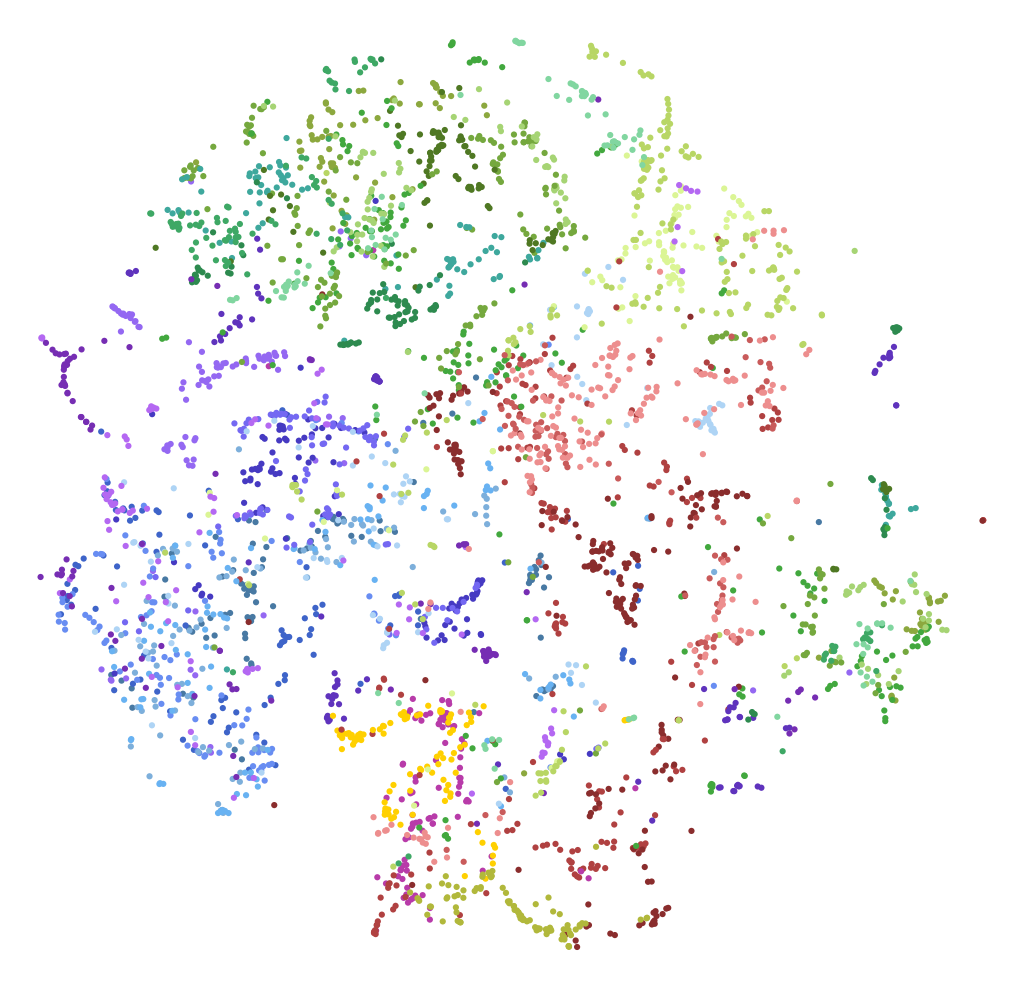
\includegraphics[width=\textwidth]{instruments-tsne.png}
	\caption{A 2-D t-SNE embedding of sounds from Vienna Symphonic Library shows that a convolutional neural network can learn a manifold that separates the sounds of woodwinds (blue colors), strings (red colors), and brass (green colors) instruments.}\label{fig:tsne}
\end{figure}




